\documentclass[10pt,a4paper,twocolumn]{article}

\usepackage[T1]{fontenc}
\usepackage[utf8]{inputenc}
\usepackage{lmodern}
\usepackage[margin=2cm,columnsep=0.7cm]{geometry}
\usepackage{amsmath,amssymb}
\usepackage{graphicx}
\usepackage{xcolor}
\usepackage{booktabs}
\usepackage{siunitx}
\usepackage[round,authoryear]{natbib}
\usepackage[colorlinks=true,
            linkcolor=blue!50!black,
            citecolor=blue!50!black,
            urlcolor=blue!50!black]{hyperref}

\graphicspath{{../figures/}}
\sisetup{per-mode=power}
\setlength{\bibsep}{2pt}

\renewcommand{\topfraction}{0.9}
\renewcommand{\dbltopfraction}{0.9}
\renewcommand{\textfraction}{0.1}
\renewcommand{\floatpagefraction}{0.8}
\renewcommand{\dblfloatpagefraction}{0.8}
\setcounter{topnumber}{3}
\setcounter{dbltopnumber}{2}

\newcommand{\Fdir}{F_\mathrm{dir}}
\newcommand{\Find}{F_\mathrm{ind}}
\newcommand{\nisn}{n_\mathrm{ISN}}
\newcommand{\au}{\mathrm{au}}

\begin{document}

\twocolumn[
\begin{@twocolumnfalse}
\begin{center}
  {\LARGE\bfseries Direct and indirect beams of interstellar helium as a
   calibration-free probe of the ionization rate\par}
  \vspace{10pt}
  {\large Kishan Deka\par}
  \vspace{4pt}
  {\small \today\par}
\end{center}

\begin{abstract}
\noindent
Pickup ions measured by New Horizons/SWAP suggest that the ionization rate of
interstellar neutral (ISN) helium is about 43\% higher than solar-proxy models
predict. Pickup-ion and direct-beam measurements cannot tell a higher
ionization rate apart from a higher interstellar density, because both scale
with their product, and the direct-beam flux also depends on a poorly known
detector efficiency. ISN helium reaches 1\,au on two kinds of orbits: a
\emph{direct} beam and an \emph{indirect} beam that first passes around the
Sun. Indirect atoms spend more time close to the Sun and are ionized more, so
the ratio of the two beam fluxes depends on the ionization rate but not on the
density or on the absolute efficiency. I build a simple analytic model of ISN
helium at 1\,au and use it to predict both beams over the year as seen by a
Sun-pointing spinning detector such as IMAP-Lo. A 43\% higher ionization rate
lowers the ratio of the late-October indirect beam to the February direct beam
by a factor of 0.61, while a 43\% higher density leaves it unchanged.
Measuring both beams therefore separates the two explanations. I discuss the
physical and instrumental effects that a full analysis would need to include.
\end{abstract}
\vspace{1.5em}
\end{@twocolumnfalse}
]

% ------------------------------------------------------------------------
\begin{figure*}[t]
  \centering
  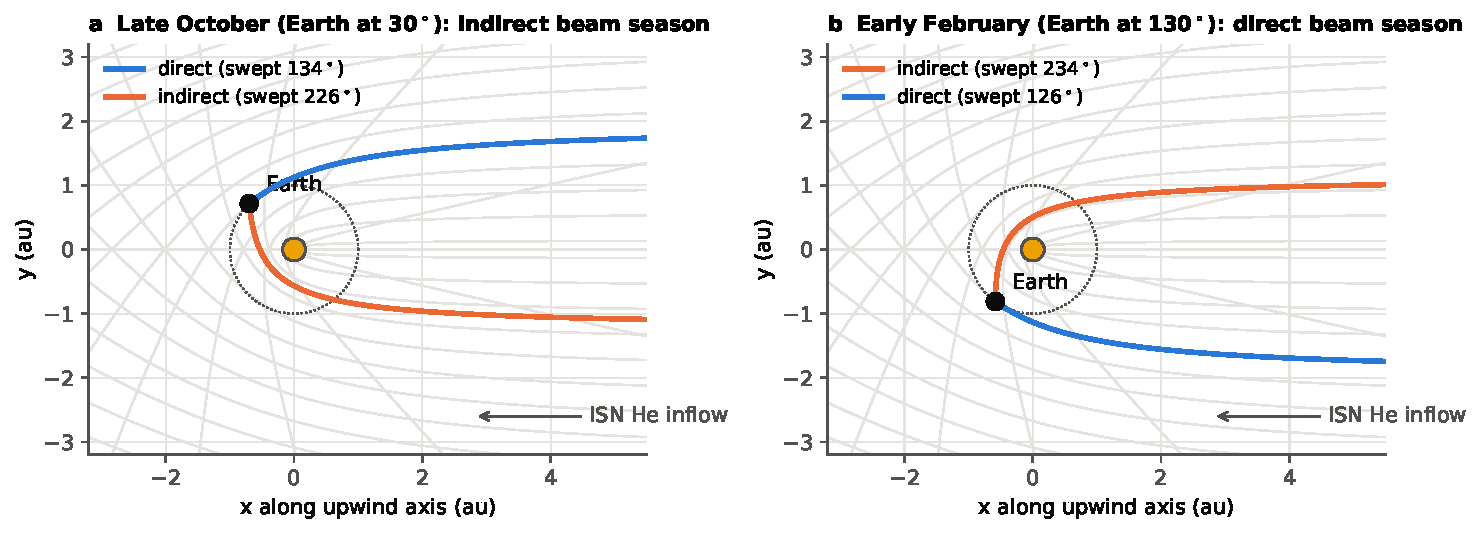
\includegraphics[width=0.9\textwidth]{fig1_trajectories.pdf}
  \caption{Direct (blue) and indirect (orange) orbits of a cold helium flow
  reaching Earth in late October (a) and early February (b), in the plane of
  the inflow. The gas arrives from the right, and the dotted circle is Earth's
  orbit. The angle each orbit has swept around the Sun is given in the
  legend.}
  \label{fig:traj}
\end{figure*}

\section{Introduction}
\label{sec:intro}

The Sun moves through the partially ionized local interstellar medium, and
the neutral part of that medium flows freely into the heliosphere. Helium is
the best-studied interstellar neutral (ISN) species. It is barely filtered at
the heliospheric boundary, and radiation pressure on it is weak, so its atoms
move on nearly Keplerian orbits and keep the imprint of the interstellar
conditions. The flow was measured by the GAS instrument on Ulysses
\citep{Witte2004} and, since 2009, by IBEX-Lo on the Interstellar Boundary
Explorer \citep{McComas2009,Fuselier2009,Mobius2009}. Analyses of the IBEX-Lo
data \citep{Bzowski2012,Lee2012} led to a consensus set of inflow parameters
\citep{McComas2015}, and revealed a slower, warmer secondary population, the
``Warm Breeze'' \citep{Kubiak2014}.

On the way in, helium atoms are lost mainly through ionization by solar EUV
radiation \citep{Sokol2019}. The ionization rate therefore sets how much
helium survives to 1\,au, and every interpretation of ISN He data depends on
it. Two recent results suggest the rate is higher than models based on solar
proxies predict. \citet{Swaczyna2022} found that the evolution of the ISN He
flux seen by IBEX-Lo over a solar cycle requires a change in detection
efficiency, a higher ionization rate, or an additional signal.
\citet{Antonik2025} derived the ionization rate from He$^+$ pickup ions
measured by New Horizons/SWAP and found it to be about 43\% higher than the
model rate.

Neither result can separate the ionization rate from the interstellar
density. Pickup-ion production is proportional to the product of density and
ionization rate. The direct-beam flux at IBEX-Lo is proportional to the
density, to the survival probability and to the absolute detection
efficiency, which is only known to tens of percent. ``More ionization'',
``more helium'' and ``a different efficiency'' are therefore largely
degenerate.

\citet{Bzowski2023} proposed a way around this: compare the fluxes of the
\emph{direct} and \emph{indirect} beams. Indirect atoms pass around the Sun
before reaching the detector, so they are exposed to ionization for longer.
In the ratio of the two beams the density and the absolute efficiency cancel,
while the ionization rate does not. Earlier attempts were limited because the
indirect beam could not be separated from the background. IMAP-Lo on the
Interstellar Mapping and Acceleration Probe \citep{McComas2018} sits on a
pivot platform that can point at the indirect beam, and \citet{Kubiak2023}
designed an observation plan that includes calibration-free determination of
the He ionization rate.

This work is a small, independent implementation of the direct/indirect-beam
idea. It asks a narrow question: if the SWAP result is right, how large is the
change in the beam ratio, and does the ratio really distinguish a higher
ionization rate from a higher density?

% ------------------------------------------------------------------------
\section{Method}
\label{sec:method}

\begin{figure}[t]
  \centering
  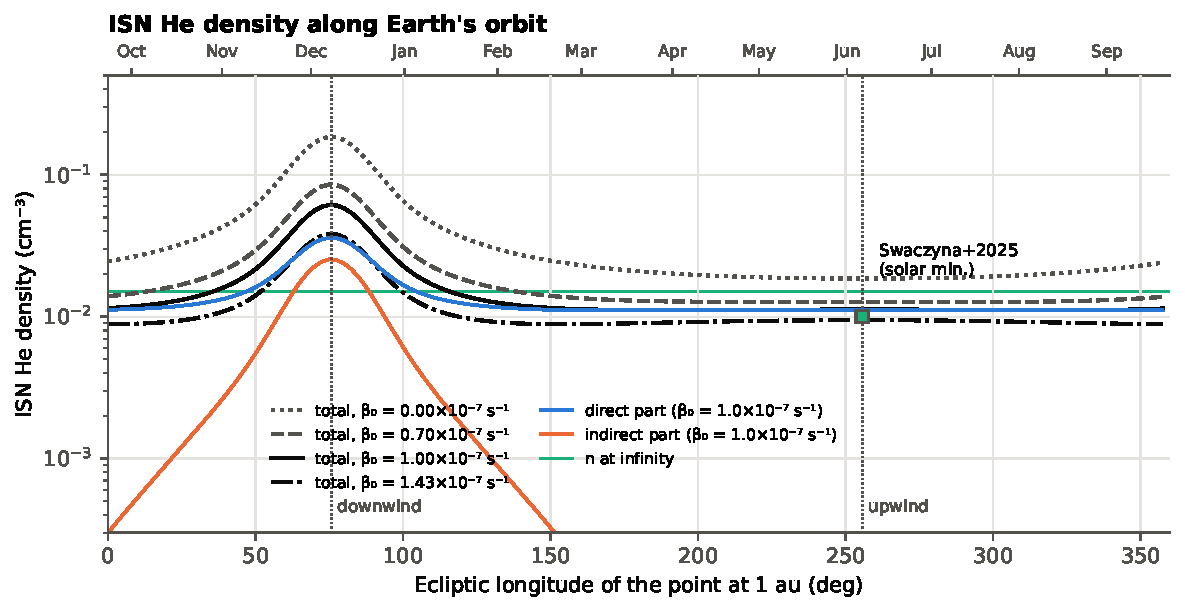
\includegraphics[width=\columnwidth]{fig2_density_1au.pdf}
  \caption{ISN He density along Earth's orbit for several ionization rates,
  and its direct and indirect parts for $\beta_0 = \SI{1e-7}{\per\second}$.
  The green line is the density far from the Sun and the square is the
  solar-minimum value of \citet{Swaczyna2025}.}
  \label{fig:dens}
\end{figure}

\begin{figure*}[t]
  \centering
  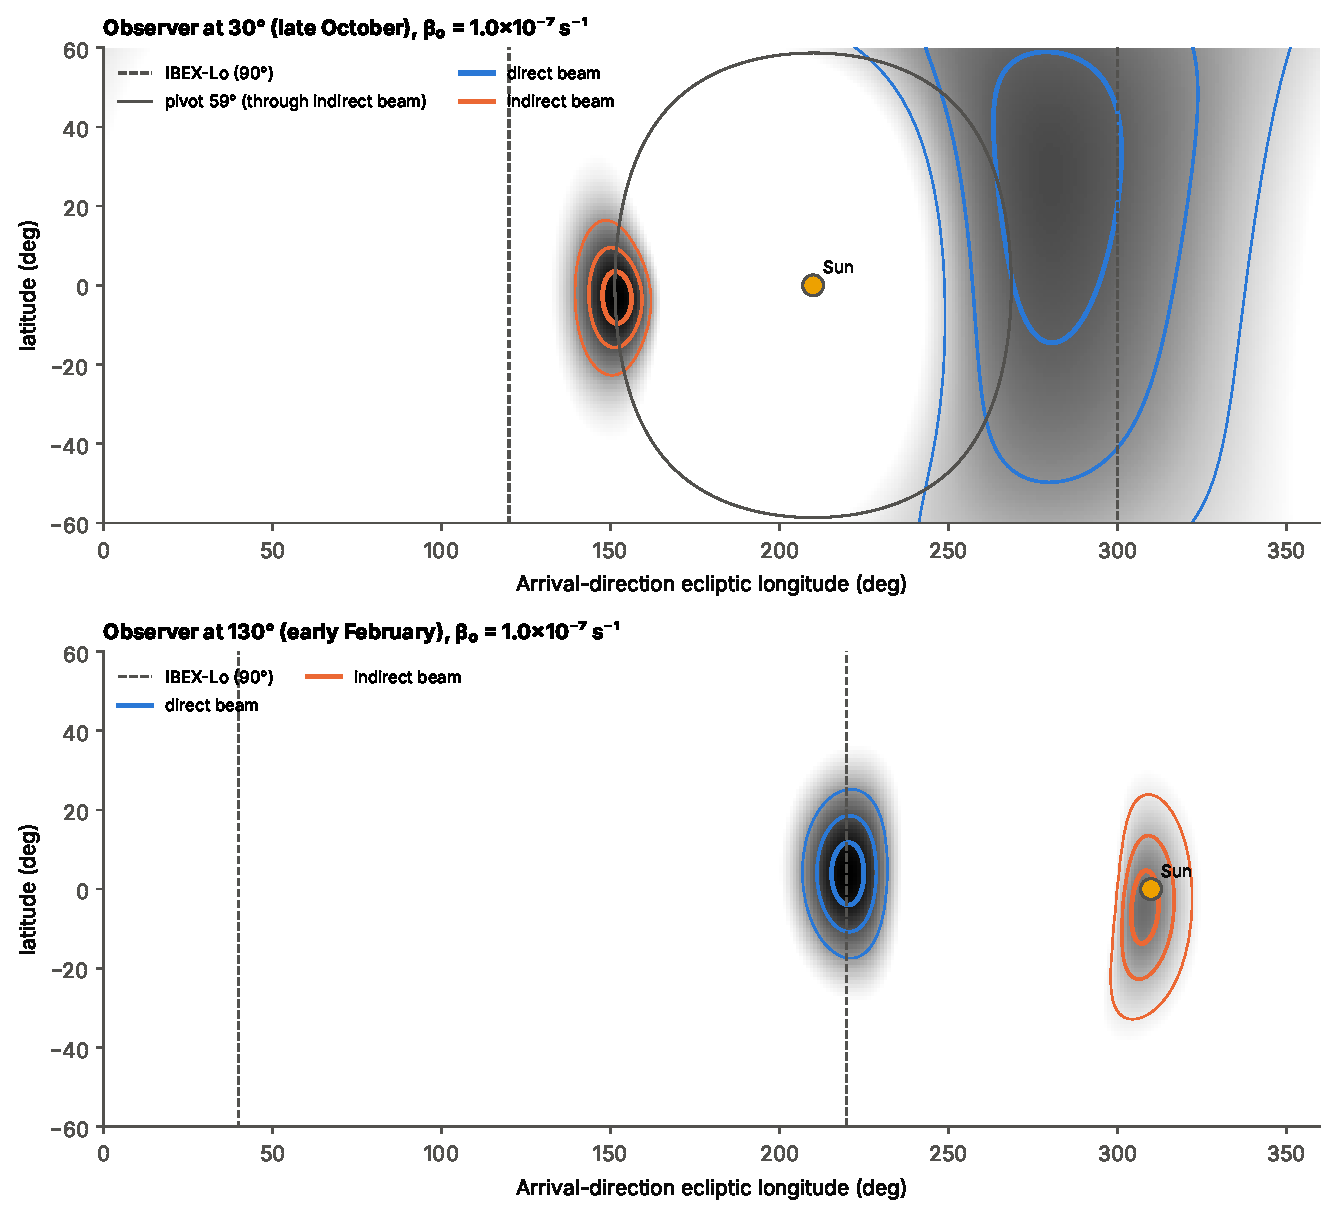
\includegraphics[width=0.75\textwidth]{fig3_skymaps.pdf}
  \caption{Helium flux on the sky seen from Earth in late October (top) and
  early February (bottom), in ecliptic coordinates of the arrival direction.
  Grey shading is the total flux; blue and orange contours trace the direct
  and indirect beams. The dashed curve is the IBEX-Lo viewing circle (\ang{90}
  from the Sun); the solid curve is the IMAP-Lo pivot angle that crosses the
  indirect beam.}
  \label{fig:sky}
\end{figure*}

\subsection{Model of ISN helium at 1\,au}

Far from the Sun the helium is a Maxwellian gas moving towards the Sun with
the inflow parameters in Table~\ref{tab:params}. Near the Sun, every atom
follows a Keplerian hyperbola under solar gravity; radiation pressure is
neglected. Two such orbits reach every point near the Sun: the \emph{direct}
orbit, which has swept less than \ang{180} around the Sun since it left
infinity, and the \emph{indirect} orbit, which has swept more than \ang{180}
(Figure~\ref{fig:traj}).

Along the way atoms are ionized at a rate that falls off with distance from
the Sun as
\begin{equation}
  \beta(r) = \beta_0\left(\frac{1\,\au}{r}\right)^2 ,
\end{equation}
where $\beta_0$ is the rate at 1\,au. For this form of $\beta(r)$ the total
exposure along a Keplerian orbit has a simple closed form, so the fraction of
atoms that survive to the observer is
\begin{equation}
  S = e^{-\beta_0 X}, \qquad X = \frac{(1\,\au)^2\,\Delta\nu}{h},
  \label{eq:survival}
\end{equation}
where $\Delta\nu$ is the angle the atom has swept since infinity and $h$ is
its angular momentum. The exposure factor $X$ has units of time and depends
only on the orbit. Indirect atoms have a larger $\Delta\nu$ and pass closer
to the Sun, so their $X$ is several times larger.

By Liouville's theorem, the velocity distribution at the observer is the
interstellar distribution evaluated on the same orbit, reduced by the survival
probability:
\begin{equation}
  f(\mathbf{r},\mathbf{v}) = f_\mathrm{LISM}(\mathbf{v}_\infty)\,e^{-\beta_0 X}.
\end{equation}
Here $\mathbf{v}_\infty$ is the velocity the atom had far from the Sun, which
follows analytically from the orbit. This is the classical ``hot model'' of
interstellar gas \citep{Thomas1978,Lee2012}. The beam flux seen by an observer
is the integral of $f$ over all arrival directions and speeds, done
separately for direct and indirect atoms. It is computed numerically on a
grid of directions and speeds, with the observer moving with Earth at
\SI{29.78}{\kilo\metre\per\second}; the results change by less than
$5\times10^{-4}$ when the grid is refined.

\subsection{Why the beam ratio measures the ionization rate}

Each beam flux is proportional to the interstellar density $\nisn$ and, once
detected, to the absolute efficiency $\varepsilon$. Its dependence on the
ionization rate is described by the beam's mean exposure
$\langle X\rangle = -\mathrm{d}\ln F/\mathrm{d}\beta_0$. For the ratio
$R = \Find/\Fdir$ of the two beams this gives, to a good approximation,
\begin{equation}
  \ln R = \mathrm{const} - \beta_0\big(\langle X\rangle_\mathrm{ind} - \langle X\rangle_\mathrm{dir}\big).
  \label{eq:ratio}
\end{equation}
The constant does not depend on $\nisn$ or $\varepsilon$, which cancel in the
ratio, but $\beta_0$ remains. A higher ionization rate lowers the ratio,
while a higher density leaves it unchanged.

\begin{table}[t]
  \centering
  \caption{Model parameters and reference values. Inflow parameters from
  \citet{McComas2015}; enhancement factor from \citet{Antonik2025}.}
  \label{tab:params}
  \small
  \begin{tabular}{@{}lr@{}}
    \toprule
    \multicolumn{2}{@{}l}{\emph{ISN He far from the Sun}} \\
    Density $\nisn$ & \SI{0.015}{\per\cubic\centi\metre} \\
    Inflow speed & \SI{25.4}{\kilo\metre\per\second} \\
    Upwind longitude, latitude & \ang{255.7}, \ang{5.1} \\
    Temperature & \SI{7500}{\kelvin} \\
    \midrule
    \multicolumn{2}{@{}l}{\emph{Ionization}} \\
    Model rate at 1\,au, $\beta_0$ & \SI{1.0e-7}{\per\second} \\
    Enhancement factor (SWAP) & 1.43 \\
    \midrule
    \multicolumn{2}{@{}l}{\emph{Observations}} \\
    Observer orbit & circular, 1\,au \\
    Direct beam & Earth at \ang{130}, early Feb. \\
    Indirect beam & Earth at \ang{30}, late Oct. \\
    \bottomrule
  \end{tabular}
\end{table}

\begin{figure*}[t]
  \centering
  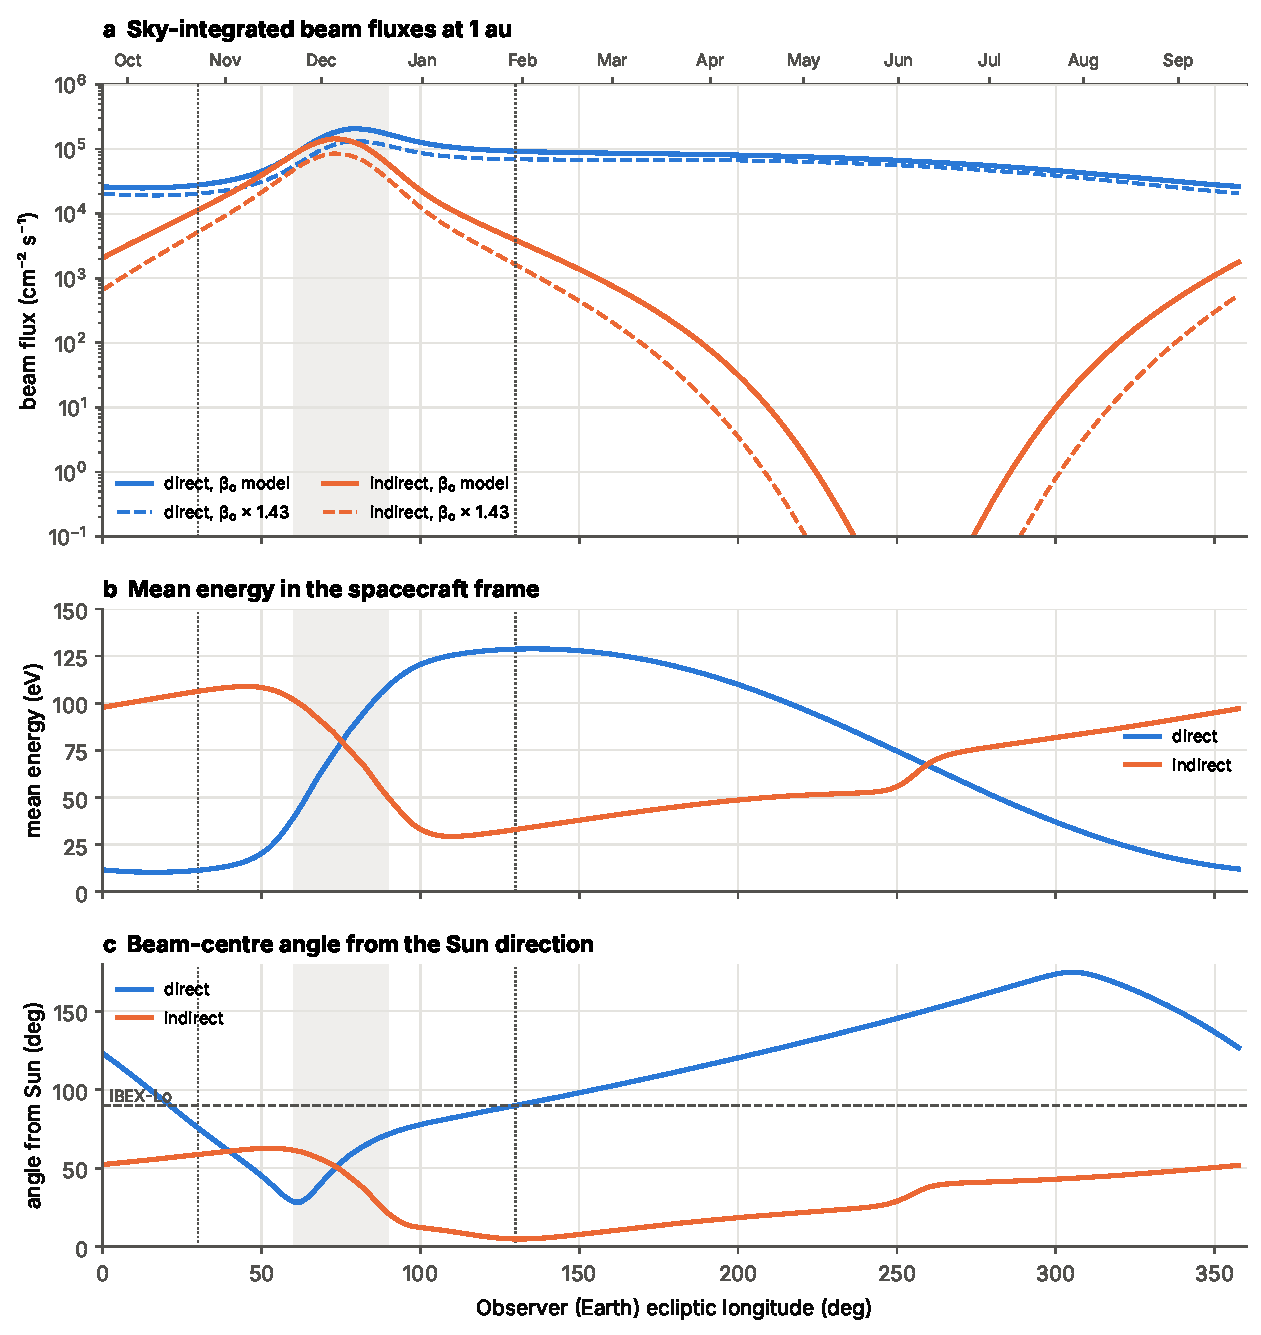
\includegraphics[width=0.62\textwidth]{fig4_annual_beams.pdf}
  \caption{The two beams over the year, against Earth's ecliptic longitude
  (months on top). (a) Beam fluxes for the model ionization rate (solid) and
  a 43\% higher rate (dashed). (b) Mean beam energy seen by the detector.
  (c) Angle between the beam centre and the Sun. Grey bands mark seasons where
  the two beams overlap on the sky; dotted lines mark the two reference
  seasons.}
  \label{fig:annual}
\end{figure*}

\subsection{Observing setup and hypotheses}

IBEX and IMAP are Sun-pointing spinning spacecraft. IBEX-Lo looks
perpendicular to the spin axis, so it scans a circle \ang{90} from the Sun,
which sees the direct beam well around February. IMAP-Lo can change this
angle with its pivot platform \citep{McComas2018,Kubiak2023}. In the model,
the angle needed to observe a beam is the angle between the beam centre and
the Sun.

The direct beam is taken at its February peak (Earth at ecliptic longitude
\ang{130}), where IBEX-Lo has measured it for over a decade. The indirect beam
is taken in late October (Earth at \ang{30}), where it is bright and well
separated from the direct beam. Two explanations of the SWAP result are
compared:
\begin{itemize}
  \item \textbf{H1}: the ionization rate is 1.43 times the model value, at
    the same density;
  \item \textbf{H2}: the density is 1.43 times higher, at the model
    ionization rate.
\end{itemize}
Both give the same pickup-ion production, so pickup ions alone cannot tell
them apart.

% ------------------------------------------------------------------------
\begin{figure*}[t]
  \centering
  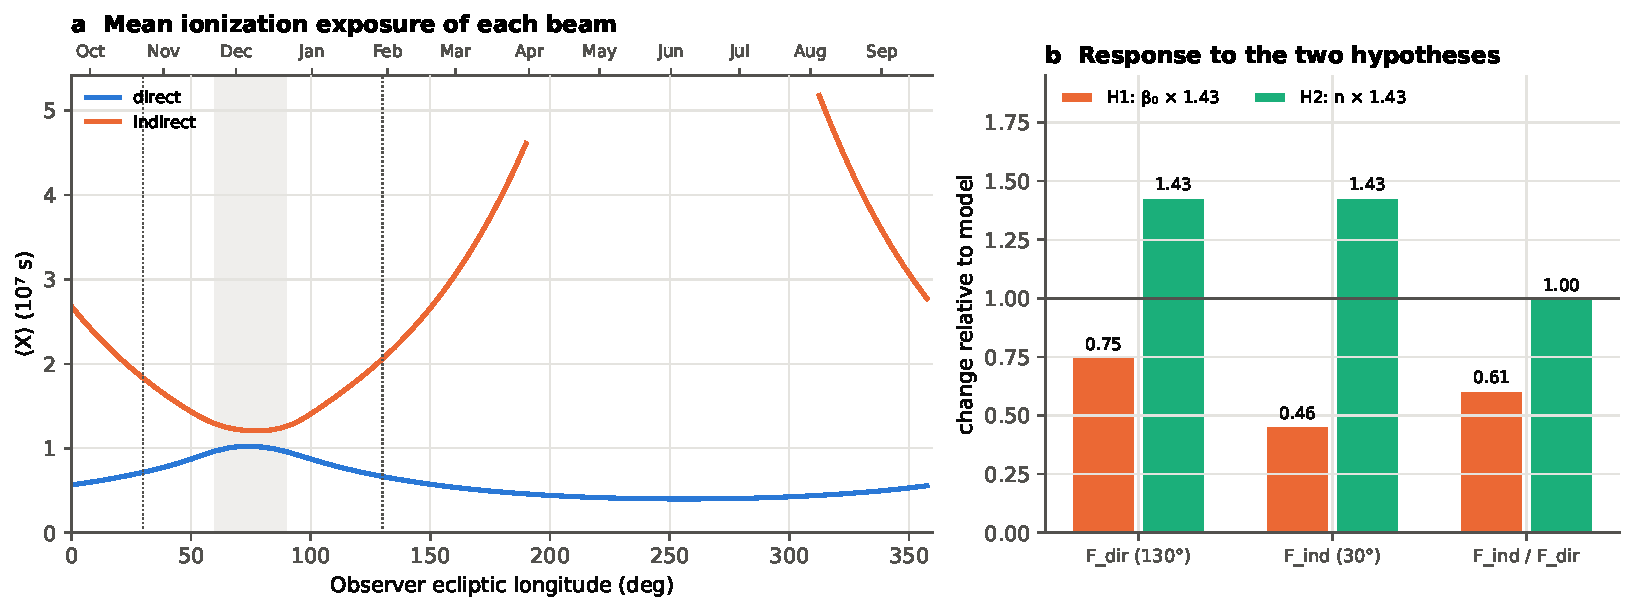
\includegraphics[width=0.95\textwidth]{fig5_exposure_response.pdf}
  \caption{(a) Mean ionization exposure $\langle X\rangle$ of each beam over
  the year. (b) Change of the February direct-beam flux, the late-October
  indirect-beam flux and their ratio under the two hypotheses, relative to the
  model.}
  \label{fig:resp}
\end{figure*}

\section{Results}
\label{sec:results}

\paragraph{Two orbits to Earth.} Figure~\ref{fig:traj} shows the two orbits
that reach Earth in the two reference seasons, for a cold flow. The indirect
orbits sweep \ang{226} (October) and \ang{234} (February) around the Sun,
compared with \ang{134} and \ang{126} for the direct ones, and pass much
closer to the Sun. That longer path near the Sun is the source of their
larger ionization exposure.

\paragraph{Model check.} The helium density along Earth's orbit
(Figure~\ref{fig:dens}) checks that the model behaves sensibly. Upwind, the
model gives \SI{0.011}{\per\cubic\centi\metre} at the model ionization rate,
close to the \SI{\approx0.01}{\per\cubic\centi\metre} adopted by
\citet{Swaczyna2025} for solar minimum. Downwind, solar gravity focuses the
atoms into a cone where the density rises more than five-fold, and about 40\% of the
atoms there are on indirect orbits.

\paragraph{Where the beams appear.} Figure~\ref{fig:sky} shows where the two
beams arrive from. In late October the indirect beam is a compact spot about
\ang{59} from the Sun. The \ang{90} IBEX-Lo circle misses it, but an IMAP-Lo
pivot angle of \ang{59} passes through its centre. In February the direct beam
sits on the IBEX-Lo circle, while the indirect beam arrives from within a few
degrees of the Sun and cannot be observed.

\begin{figure}[t]
  \centering
  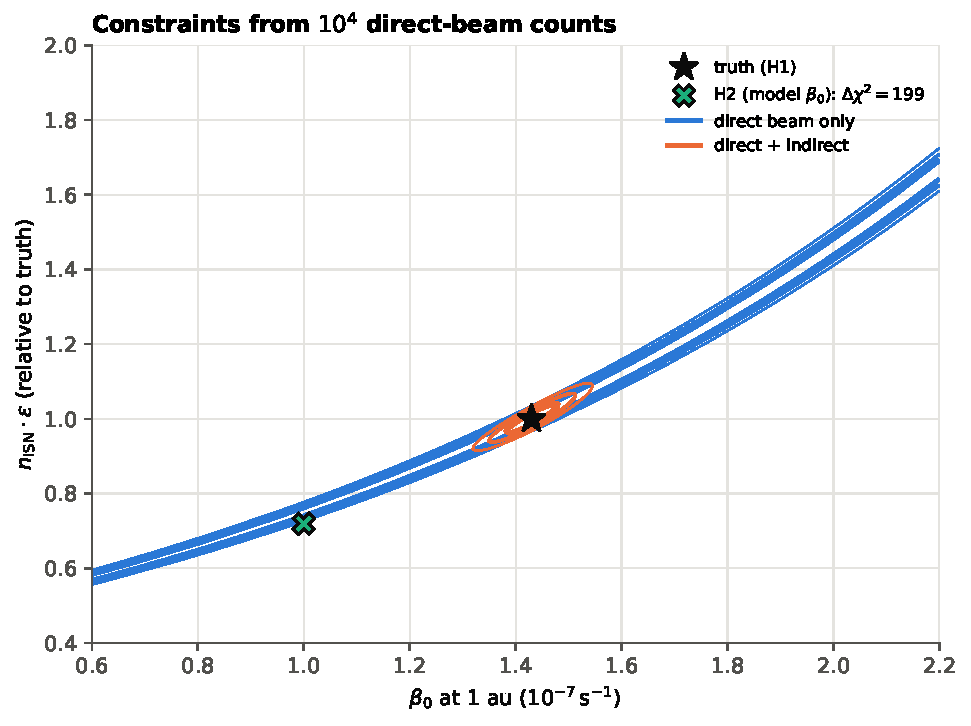
\includegraphics[width=\columnwidth]{fig6_degeneracy.pdf}
  \caption{Constraints on the ionization rate $\beta_0$ and on the product of
  density and detector efficiency, $\nisn\varepsilon$, from noise-free
  simulated counts generated under H1 (star). Blue: direct beam only; orange:
  direct and indirect beams together. Contours are the 1, 2 and $3\sigma$
  levels. The cross marks H2.}
  \label{fig:degen}
\end{figure}

\paragraph{The beams over the year.} Figure~\ref{fig:annual} follows both
beams around Earth's orbit. The direct beam is bright all year. The indirect
beam is comparable to it in November and December, fades through spring, and
is negligible around June. From late November to late December the two
beams overlap on the sky and cannot be separated. In autumn the indirect beam
arrives at \SIrange{100}{110}{\electronvolt}, compared with
\SI{\approx130}{\electronvolt} for the February direct beam. It stays
\ang{50}--\ang{60} from the Sun, so it needs a pivot angle well below
\ang{90}. In every season the indirect beam responds more strongly to the
ionization rate (panel a).

\paragraph{The ratio separates the hypotheses.} This is the main result
(Figure~\ref{fig:resp}). The indirect beam accumulates 1.5 to 5 times more
exposure than the direct beam, with the largest contrast early in autumn. For
the reference pair the mean exposures are \SI{0.67e7}{\second} (direct,
February) and \SI{1.83e7}{\second} (indirect, October). Under H1, the
higher ionization rate lowers the direct beam to 0.75 and the indirect beam to
0.46 of the model, so the ratio drops to 0.61. Under H2, both beams rise by
1.43 and the ratio stays exactly the same. The absolute direct-beam flux alone
could only separate the two if the detector efficiency were known to much
better than the 25--43\% difference between them. The ratio does not need it.

\paragraph{Breaking the degeneracy.} Figure~\ref{fig:degen} shows the same
point as a fit. Noise-free counts are simulated under H1, with $10^4$ counts
in the February direct beam and about 750 in the October indirect beam for the
same exposure time. They are then fitted for $\beta_0$ and the unknown
product $\nisn\varepsilon$, using a Poisson likelihood
\citep{BakerCousins1984}. The direct beam alone only constrains a curved band:
a higher ionization rate can always be traded for more helium or a more
efficient detector. Adding the indirect beam closes the contour around the
true values, and H2 is strongly disfavoured ($\Delta\chi^2\approx199$). This
idealized test shows how the second beam lifts the degeneracy. It is not a
forecast of the achievable precision, which depends on the effects discussed
next.

% ------------------------------------------------------------------------
\section{Limitations and future work}
\label{sec:limits}

The model is a feasibility study of the size of the beam-ratio signal. A full
analysis of IMAP-Lo data would need the following, roughly in order of
importance.

\paragraph{Radiation pressure.} The orbits are purely Keplerian.
\citet{KowalskaLeszczynska2023} showed that radiation pressure changes the
IMAP-Lo helium fluxes by up to 9\% for the indirect beam, likely more than the
statistical uncertainty. Including it requires numerical orbits, since the
closed form of Equation~(\ref{eq:survival}) no longer holds.

\paragraph{Other near-Sun losses.} The ratio measures the \emph{total} extra
loss of indirect atoms, not photoionization alone. Elastic scattering by
solar-wind particles has been proposed as an alternative to a higher
ionization rate \citep{ElasticScattering2024}, and it would lower the ratio
in the same way. Separating the two would rely on their different energy and
angular signatures.

\paragraph{Secondary helium.} The Warm Breeze \citep{Kubiak2014} arrives from
a different direction and has its own direct and indirect beams, which must be
added to the model.

\paragraph{Time-dependent and non-$r^{-2}$ ionization.} Indirect atoms spend
months near the Sun, and the two beams are observed months apart, so
solar-cycle changes of the ionization rate matter. Electron-impact ionization
does not fall off as $r^{-2}$ \citep{Sokol2019}. Both effects need a numerical
exposure integral along each orbit.

\paragraph{Instrument response.} The model uses sky-integrated fluxes. A
realistic prediction needs the IMAP-Lo collimator, the pivot schedule
\citep{Kubiak2023} and the energy-dependent detection efficiency. Since the
two reference beams arrive about 20\% apart in energy, an energy-dependent
efficiency does not fully cancel in their ratio. Choosing pairs of
observations at matched energies, as recommended by \citet{Bzowski2023}, would
reduce this effect. A first look at a simple energy threshold is in progress.

\paragraph{Inflow-parameter uncertainties and counting statistics.} The
uncertainties of the inflow speed, direction and temperature
\citep{McComas2015} also move the beam ratio, and the number of counts
needed to detect the signal depends on the observing season. These are being
estimated. Since the inflow parameters are derived from direct-beam data and
are correlated, the natural approach is a joint fit of the inflow parameters
and the ionization rate to both beams.

% ------------------------------------------------------------------------
\section{Summary}
\label{sec:summary}

A simple analytic model of interstellar helium at 1\,au confirms that the
ratio of the indirect to the direct beam is a sensitive, calibration-free
measure of the helium ionization rate. If the ionization rate is 43\% higher
than models predict, as New Horizons/SWAP pickup ions suggest, the ratio of
the late-October indirect beam to the February direct beam drops by about
40\%. A 43\% higher interstellar density leaves the ratio unchanged. The
indirect beam is bright and well separated in autumn, about \ang{60} from the
Sun, where IMAP-Lo's pivot platform can observe it. Radiation pressure,
additional near-Sun losses, secondary helium and the instrument response are
the main effects to add before the method can be applied to real data.

\section*{Code availability}

The model, the scripts that generate the data and the notebook that makes the
figures are in the project repository (\texttt{src/isnhe},
\texttt{scripts/}, \texttt{notebooks/plot\_figures.ipynb}).

% ------------------------------------------------------------------------
{\small
\begin{thebibliography}{99}
\providecommand{\natexlab}[1]{#1}

\bibitem[{Antonik} et~al.(2025)]{Antonik2025}
Antonik, M., Swaczyna, P., McComas, D.~J., Elliott, H.~A., \& Bzowski, M.
  2025, ApJ, 995, 57

\bibitem[{Baker} \& {Cousins}(1984)]{BakerCousins1984}
Baker, S., \& Cousins, R.~D. 1984, Nucl. Instrum. Methods Phys. Res., 221, 437

\bibitem[{Bzowski} et~al.(2012)]{Bzowski2012}
Bzowski, M., Kubiak, M.~A., M\"obius, E., et~al. 2012, ApJS, 198, 12

\bibitem[{Bzowski} et~al.(2023)]{Bzowski2023}
Bzowski, M., Kubiak, M.~A., M\"obius, E., \& Schwadron, N.~A. 2023, ApJS,
  265, 24

\bibitem[{arXiv:2409.11784}(2024)]{ElasticScattering2024}
\textit{IBEX Observations of Elastic Scattering of Interstellar Helium by
  Solar Wind Particles}, 2024, arXiv:2409.11784

\bibitem[{Fuselier} et~al.(2009)]{Fuselier2009}
Fuselier, S.~A., Bochsler, P., Chornay, D., et~al. 2009, SSRv, 146, 117

\bibitem[{Kowalska-Leszczy\'nska} et~al.(2023)]{KowalskaLeszczynska2023}
Kowalska-Leszczy\'nska, I., Kubiak, M.~A., \& Bzowski, M. 2023, ApJ, 950, 98

\bibitem[{Kubiak} et~al.(2014)]{Kubiak2014}
Kubiak, M.~A., Bzowski, M., Sok\'o\l, J.~M., et~al. 2014, ApJS, 213, 29

\bibitem[{Kubiak} et~al.(2023)]{Kubiak2023}
Kubiak, M.~A., Bzowski, M., et~al. 2023, ApJS, arXiv:2309.06931

\bibitem[{Lee} et~al.(2012)]{Lee2012}
Lee, M.~A., Kucharek, H., M\"obius, E., et~al. 2012, ApJS, 198, 10

\bibitem[{McComas} et~al.(2009)]{McComas2009}
McComas, D.~J., Allegrini, F., Bochsler, P., et~al. 2009, SSRv, 146, 11

\bibitem[{McComas} et~al.(2015)]{McComas2015}
McComas, D.~J., Bzowski, M., Fuselier, S.~A., et~al. 2015, ApJS, 220, 22

\bibitem[{McComas} et~al.(2018)]{McComas2018}
McComas, D.~J., Christian, E.~R., Schwadron, N.~A., et~al. 2018, SSRv, 214,
  116

\bibitem[{M\"obius} et~al.(2009)]{Mobius2009}
M\"obius, E., Bochsler, P., Bzowski, M., et~al. 2009, Science, 326, 969

\bibitem[{Sok\'o\l} et~al.(2019)]{Sokol2019}
Sok\'o\l, J.~M., Bzowski, M., \& Tokumaru, M. 2019, ApJ, 872, 57

\bibitem[{Swaczyna} et~al.(2022)]{Swaczyna2022}
Swaczyna, P., Kubiak, M.~A., Bzowski, M., et~al. 2022, ApJS, 259, 42

\bibitem[{Swaczyna} et~al.(2025)]{Swaczyna2025}
Swaczyna, P., Bzowski, M., \& Kubiak, M.~A. 2025, ApJS, 277, 17

\bibitem[{Thomas}(1978)]{Thomas1978}
Thomas, G.~E. 1978, Annu. Rev. Earth Planet. Sci., 6, 173

\bibitem[{Witte}(2004)]{Witte2004}
Witte, M. 2004, A\&A, 426, 835

\end{thebibliography}
}

\end{document}
